\documentclass[12pt, a4paper]{article}
\usepackage[margin=1in]{geometry}
\usepackage{amsmath}
\usepackage{amssymb}
\usepackage{graphicx}
\usepackage{hyperref}
\usepackage{tikz}
\usetikzlibrary{decorations.pathmorphing} % For drawing photons
\usepackage{siunitx} % For SI units
\usepackage{caption} % For better figure captioning

\title{The Bohr Model \& Atomic Energy Levels: \\ A Comprehensive Guide with Solved Problems}
\author{}
\date{\today}

\begin{document}
\maketitle

\section*{Part 1: Theoretical Notes}

The Bohr model, proposed by Niels Bohr in 1913 and later refined by Louis de Broglie, provides a foundational framework for understanding atomic structure and spectra. It successfully explains the stability of atoms and the discrete nature of their emitted light by introducing several revolutionary postulates.

\subsection*{Key Postulates \& Concepts}
\begin{enumerate}
    \item \textbf{Stationary States:} Electrons revolve around the nucleus in specific, discrete circular orbits called "stationary states" without radiating energy. Each state corresponds to a fixed energy level.

    \item \textbf{Quantization of Angular Momentum:} The angular momentum ($L$) of an electron in a stationary state is quantized. It can only take on integer multiples of $\frac{h}{2\pi}$ (where $h$ is Planck's constant).
    $$ L = m_e v r = n \frac{h}{2\pi} $$
    Here, $n$ is the principal quantum number ($n=1, 2, 3, \dots$). This condition restricts the possible radii and velocities of the electron.

    \item \textbf{de Broglie's Hypothesis and Standing Waves:} Louis de Broglie proposed that particles, like electrons, have wave-like properties. An electron's orbit is stable only if its circumference is an integer multiple of its wavelength ($\lambda_{dB}$). This creates a constructive standing wave pattern.
    $$ 2\pi r = n\lambda_{dB}, \quad \text{where } \lambda_{dB} = \frac{h}{p} = \frac{h}{m_e v} $$
    Substituting $\lambda_{dB}$ into the circumference condition directly yields the Bohr's quantization of angular momentum: $2\pi r = n(\frac{h}{m_e v}) \implies m_e v r = n\frac{h}{2\pi}$.

    \begin{figure}[h!]
    \centering
    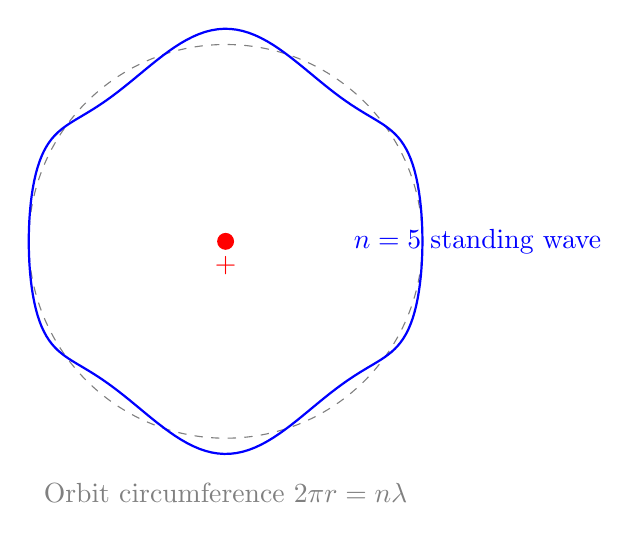
\begin{tikzpicture}
        % Orbit
        \draw[dashed, gray] (0,0) circle (2.5cm);
        % Nucleus
        \filldraw[red] (0,0) circle (0.1cm) node[below=2pt]{+};
        % Standing wave
        \draw[blue, thick, domain=0:360, samples=200] plot ({2.5*cos(\x)}, {2.5*sin(\x) + 0.2*sin(5*\x)});
        \node[blue] at (3.2, 0) {$n=5$ standing wave};
        \node[gray] at (0, -3.2) {Orbit circumference $2\pi r = n\lambda$};
    \end{tikzpicture}
    \caption{de Broglie's standing wave condition for a stable electron orbit.}
    \end{figure}

    \item \textbf{Energy Transitions:} An electron can "jump" between energy levels by absorbing or emitting a photon. The photon's energy must exactly match the energy difference between the initial ($E_i$) and final ($E_f$) states.
    $$ E_{\text{photon}} = |\Delta E| = |E_f - E_i| $$
    
    \begin{figure}[h!]
    \centering
    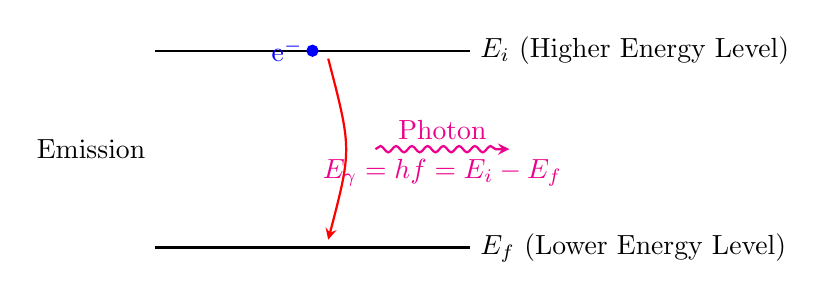
\begin{tikzpicture}[>=stealth]
        % Energy levels
        \draw[thick] (-2, 2.5) -- (2, 2.5) node[right] {$E_i$ (Higher Energy Level)};
        \draw[thick] (-2, 0) -- (2, 0) node[right] {$E_f$ (Lower Energy Level)};
        
        % Electron transition
        \filldraw[blue] (0, 2.5) circle (2pt);
        \draw[->, thick, red] (0.2, 2.4) .. controls (0.5, 1.25) .. (0.2, 0.1);
        \node[left, blue] at (0, 2.5) {e$^-$};
        
        % Emitted photon
        \draw[->, thick, magenta, decorate, decoration={snake,amplitude=0.4mm,segment length=2mm,post length=1mm}] (0.8, 1.25) -- (2.5, 1.25);
        \node[above, magenta] at (1.65, 1.25) {Photon};
        \node[below, magenta] at (1.65, 1.25) {$E_{\gamma} = hf = E_i - E_f$};
        
        \node[left] at (-2, 1.25) {Emission};
    \end{tikzpicture}
    \caption{Diagram of an electron emitting a photon as it transitions to a lower energy level.}
    \end{figure}
    
\end{enumerate}


\subsection*{Key Equations with Examples}

\subsubsection*{Quantized Angular Momentum}
$$ L = n \frac{h}{2\pi} $$
\textbf{Example:} What is the orbital angular momentum of an electron in the first excited state ($n=2$) of a hydrogen atom?
$$ L = 2 \cdot \frac{6.626 \times 10^{-34} \text{ J}\cdot\text{s}}{2\pi} \approx 2.11 \times 10^{-34} \text{ J}\cdot\text{s} $$
Alternatively, this is often expressed simply as $L = \frac{h}{\pi}$.

\subsubsection*{de Broglie Wavelength of an Electron}
$$ \lambda_{dB} = \frac{h}{p} = \frac{h}{m_e v} $$
\textbf{Example:} An electron has a kinetic energy of 10 eV. What is its de Broglie wavelength?
\begin{enumerate}
    \item Convert energy to Joules: $K = 10 \text{ eV} \times 1.602 \times 10^{-19} \text{ J/eV} = 1.602 \times 10^{-18} \text{ J}$.
    \item Find momentum: $K = p^2/(2m_e) \implies p = \sqrt{2m_e K} = \sqrt{2(9.11 \times 10^{-31})(1.602 \times 10^{-18})} \approx 1.71 \times 10^{-24}$ kg m/s.
    \item Calculate wavelength: $\lambda_{dB} = \frac{h}{p} = \frac{6.626 \times 10^{-34}}{1.71 \times 10^{-24}} \approx 3.88 \times 10^{-10} \text{ m} = 0.388 \text{ nm}$.
\end{enumerate}


\subsubsection*{Energy of an Electron in a Hydrogen-like Atom}
$$ E_n = -\frac{13.6 \cdot Z^2}{n^2} \text{ eV} $$
\textbf{Example:} Find the energy of an electron in the ground state (n=1) of a singly ionized helium atom (He$^{+}$, Z=2).
$$ E_1 = -\frac{13.6 \cdot 2^2}{1^2} = -54.4 \text{ eV} $$

\subsubsection*{Energy of an Emitted/Absorbed Photon}
$$ E_{\text{photon}} = hf = \frac{hc}{\lambda} \quad (hc \approx 1240 \text{ eV}\cdot\text{nm}) $$
\textbf{Example:} An electron in a hydrogen atom falls from the n=3 state to the n=2 state. Find the photon's wavelength.
$$ E_{\text{photon}} = E_3 - E_2 = \left(-\frac{13.6}{3^2}\right) - \left(-\frac{13.6}{2^2}\right) = -1.51 - (-3.40) = 1.89 \text{ eV} $$
$$ \lambda = \frac{hc}{E_{\text{photon}}} = \frac{1240 \text{ eV}\cdot\text{nm}}{1.89 \text{ eV}} \approx 656 \text{ nm} $$


\newpage
\section*{Part 2: Original Problems and Solutions}
\hrulefill

\subsection*{Problem 1 (SPhO 2023)}
\begin{quote}
A hydrogen atom is initially at rest. An electron in the hydrogen atom makes a transition from the state with $n=3$ to the state with $n=1$. Calculate the recoil speed and recoil energy of the hydrogen during the process. [Mass of hydrogen atom is $1.66\times10^{-27}$ kg]
\end{quote}

\textbf{Solution:}
\begin{enumerate}
    \item \textbf{Calculate Photon Energy:}
    $E_{\gamma} = E_3 - E_1 = 13.6 \left(1 - \frac{1}{9}\right) \approx 12.09 \text{ eV} \approx 1.936 \times 10^{-18} \text{ J}$.
    \item \textbf{Calculate Photon Momentum:}
    $p_{\gamma} = \frac{E_{\gamma}}{c} = \frac{1.936 \times 10^{-18}}{3 \times 10^8} \approx 6.453 \times 10^{-27}$ kg m/s.
    \item \textbf{Conservation of Momentum:} $|p_{\text{atom}}| = |p_{\gamma}|$.
    \item \textbf{Calculate Recoil Speed:}
    $v_{\text{recoil}} = \frac{p_{\text{atom}}}{m_H} = \frac{6.453 \times 10^{-27}}{1.66 \times 10^{-27}} \approx 3.89$ m/s.
    \item \textbf{Calculate Recoil Energy:}
    $E_{\text{recoil}} = \frac{1}{2} m_H v^2 = \frac{(6.453 \times 10^{-27})^2}{2(1.66 \times 10^{-27})} \approx 1.25 \times 10^{-26}$ J.
\end{enumerate}
\textbf{Final Answers:} Recoil Speed: \textbf{3.89 m/s}, Recoil Energy: \textbf{$1.25 \times 10^{-26}$ J}

\hrulefill
\subsection*{Problem 2 (SPhO 2020)}
\begin{quote}
A free electron collides with a hydrogen atom in the ground state. After collision, the H atom is excited and de-excites by emitting two photons. One photon has $\lambda=656.3$ nm. The scattered electron has a de Broglie wavelength of 1.915 nm.
(a) What is the wavelength of the other photon? (b) What was the speed of the free electron before collision?
\end{quote}

\textbf{Solution:}
\begin{description}
    \item[(a) Wavelength of the other photon:]
    A photon with $\lambda=656.3$ nm corresponds to the $n=3 \to n=2$ transition. Since two photons are emitted in a cascade to the ground state ($n=1$), the full path must be $3 \to 2 \to 1$. This means the collision excited the atom to the $n=3$ level. The other photon corresponds to the $n=2 \to n=1$ transition.
    $$ \Delta E_{2 \to 1} = 13.6 \left(1 - \frac{1}{4}\right) = 10.2 \text{ eV} $$
    $$ \lambda_2 = \frac{hc}{\Delta E_{2 \to 1}} = \frac{1240}{10.2} \approx 121.6 \text{ nm} $$

    \item[(b) Speed before collision:]
    \begin{enumerate}
        \item Energy to excite H atom: $\Delta E_{1 \to 3} = 13.6(1 - 1/9) \approx 12.09$ eV.
        \item Final KE of electron: From $\lambda_{dB} = 1.915$ nm, we find its momentum $p = h/\lambda_{dB} \approx 3.46 \times 10^{-25}$ kg m/s. Then $K_{\text{final}} = p^2/(2m_e) \approx 6.57 \times 10^{-20} \text{ J} \approx 0.41$ eV.
        \item Initial KE of electron (Energy Conservation): $K_{\text{initial}} = \Delta E_{1 \to 3} + K_{\text{final}} = 12.09 + 0.41 = 12.50$ eV.
        \item Initial speed: $K_{\text{initial}} = 12.50 \text{ eV} \approx 2.00 \times 10^{-18}$ J.
        $$ v_{\text{initial}} = \sqrt{\frac{2K_{\text{initial}}}{m_e}} = \sqrt{\frac{2(2.00 \times 10^{-18})}{9.11 \times 10^{-31}}} \approx 2.09 \times 10^6 \text{ m/s} $$
    \end{enumerate}
\end{description}
\textbf{Final Answers:} (a) Wavelength: \textbf{121.6 nm}, (b) Speed: \textbf{$2.09 \times 10^6$ m/s}

\hrulefill
\subsection*{Problem 3 (SPhO 2019)}
\begin{quote}
An electron with speed $2.08 \times 10^6$ m/s collides with a stationary hydrogen atom with orbital angular momentum $L=h/\pi$. What are the possible wavelengths of photons emitted after collision?
\end{quote}

\textbf{Solution:}
\begin{enumerate}
    \item \textbf{Initial State of H atom:} From $L = n(h/2\pi)$, we find $n=2$. The atom is in the first excited state.
    \item \textbf{KE of electron:} $K_e = \frac{1}{2}m_e v^2 = \frac{1}{2}(9.11 \times 10^{-31})(2.08 \times 10^6)^2 \approx 1.97 \times 10^{-18}$ J $\approx 12.3$ eV.
    \item \textbf{Possible Excitations:} The ionization energy from $n=2$ is $3.4$ eV. Since $12.3 \text{ eV} > 3.4 \text{ eV}$, the electron can excite the atom to any higher level.
    \item \textbf{Possible Emissions:} Assuming excitation to $n=3$, the possible de-excitations are $3 \to 1$ ($\lambda \approx 102.6$ nm), $3 \to 2$ ($\lambda \approx 656.3$ nm), and the subsequent $2 \to 1$ ($\lambda \approx 121.6$ nm).
\end{enumerate}
\textbf{Final Answer:} The most prominent possible wavelengths are \textbf{102.6 nm}, \textbf{121.6 nm}, and \textbf{656.3 nm}.

\hrulefill
\subsection*{Problem 4 (SPhO 2018)}
\begin{quote}
A neutron (KE=68.2 eV) collides inelastically with a stationary He$^{+}$ ion (ground state). The neutron is scattered at 90$^{\circ}$. Find the allowed kinetic energies of the scattered particles. [$m_{He} = 4m_n$]
\end{quote}

\begin{figure}[h!]
\centering
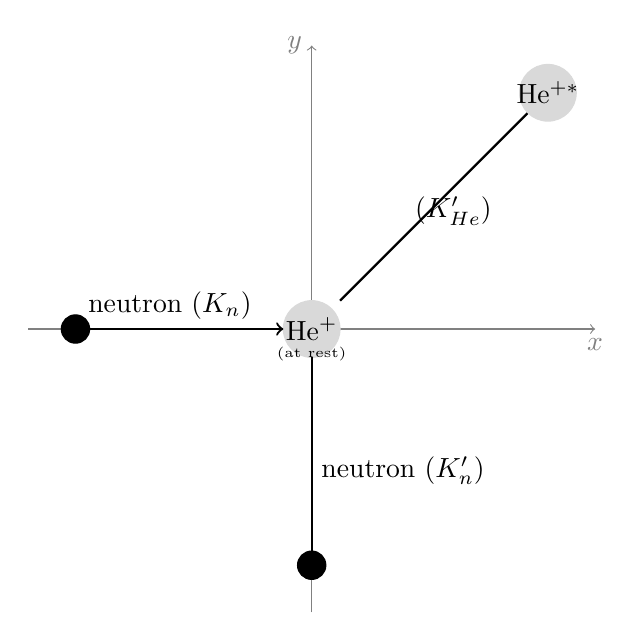
\begin{tikzpicture}[scale=1.2]
    % Axes
    \draw[->, gray] (-3,0) -- (3,0) node[below] {$x$};
    \draw[->, gray] (0,-3) -- (0,3) node[left] {$y$};
    
    % Initial He+ at rest
    \filldraw[gray!30] (0,0) circle (0.3cm);
    \node at (0,0) {He$^{+}$};
    \node[below=0.1cm] at (0,0) {\tiny (at rest)};
    
    % Incident neutron
    \draw[->, thick] (-2.5,0) -- (-0.3,0);
    \filldraw[black] (-2.5,0) circle (0.15cm);
    \node[above] at (-1.5,0) {neutron ($K_n$)};
    
    % Scattered neutron
    \draw[->, thick] (0,-0.3) -- (0,-2.5);
    \filldraw[black] (0,-2.5) circle (0.15cm);
    \node[right] at (0,-1.5) {neutron ($K_n'$)};
    
    % Recoiling He+
    \draw[->, thick] (0.3,0.3) -- (2.5,2.5);
    \filldraw[gray!30] (2.5,2.5) circle (0.3cm);
    \node at (2.5,2.5) {He$^{+*}$};
    \node[below] at (1.5,1.5) {($K_{He}'$)};
\end{tikzpicture}
\caption{Diagram of the neutron-He$^{+}$ collision.}
\end{figure}

\textbf{Solution:}
\begin{enumerate}
    \item \textbf{Conservation of Momentum} (x and y components) gives the relation: $4K'_{He} = K_n + K_n'$.
    \item \textbf{Conservation of Energy} gives: $K_n = K_n' + K'_{He} + \Delta E$.
    \item Combining these, we find a relation for the final neutron energy: $3K_n - 5K_n' = 4\Delta E$.
    \item \textbf{Allowed Excitations ($\Delta E$):} For He$^{+}$ (Z=2), $\Delta E = 54.4(1 - 1/n'^2)$. Since $K_n' > 0$, we must have $3K_n > 4\Delta E \implies 204.6 > 4\Delta E \implies \Delta E < 51.15$ eV. This allows excitations to $n'=2, 3, 4$.
    \item \textbf{Calculate Final Energies for each case:}
    \begin{itemize}
        \item \textbf{n'=2 ($\Delta E = 40.8$ eV):} $K_n' = \textbf{8.28 eV}$, $K_{He}' = \textbf{19.12 eV}$.
        \item \textbf{n'=3 ($\Delta E \approx 48.36$ eV):} $K_n' \approx \textbf{2.23 eV}$, $K_{He}' \approx \textbf{17.61 eV}$.
        \item \textbf{n'=4 ($\Delta E = 51.0$ eV):} $K_n' = \textbf{0.12 eV}$, $K_{He}' = \textbf{17.08 eV}$.
    \end{itemize}
\end{enumerate}
\textbf{Final Answer:} The allowed pairs of kinetic energies ($K_n'$, $K_{He}'$) are: \textbf{(8.28 eV, 19.12 eV)}, \textbf{(2.23 eV, 17.61 eV)}, and \textbf{(0.12 eV, 17.08 eV)}.

\newpage
\section*{Part 3: New Practice Problems and Solutions}
\hrulefill

\subsection*{Problem 1: Recoil of an Ion}
\begin{quote}
A doubly ionized lithium atom (Li$^{2+}$, Z=3) is at rest in its first excited state (n=2). It de-excites to the ground state (n=1) by emitting a single photon. Calculate the recoil velocity of the ion. [Mass of a lithium ion is approximately $1.15 \times 10^{-26}$ kg]
\end{quote}

\textbf{Solution:}
\begin{enumerate}
    \item \textbf{Calculate Photon Energy:} For Li$^{2+}$, Z=3. $E_2 = -13.6 \frac{3^2}{2^2} = -30.6$ eV. $E_1 = -13.6 \frac{3^2}{1^2} = -122.4$ eV. $E_{\gamma} = |E_1 - E_2| = 91.8$ eV.
    \item \textbf{Calculate Photon Momentum:} $E_{\gamma} \approx 1.47 \times 10^{-17}$ J. $p_{\gamma} = E_{\gamma}/c \approx 4.90 \times 10^{-26}$ kg m/s.
    \item \textbf{Conservation of Momentum:} $p_{ion} = p_{\gamma}$.
    \item \textbf{Calculate Recoil Velocity:} $v_{recoil} = p_{ion}/m_{Li} = (4.90 \times 10^{-26}) / (1.15 \times 10^{-26}) \approx 4.26$ m/s.
\end{enumerate}
\textbf{Final Answer:} The recoil velocity of the lithium ion is approximately \textbf{4.26 m/s}.

\hrulefill
\subsection*{Problem 2: Multi-Photon Emission After Collision}
\begin{quote}
A hydrogen atom, initially in its ground state, absorbs a photon and is excited. It then de-excites back to the ground state by emitting two photons in sequence. The second photon emitted has an energy of 1.89 eV.
(a) To which energy level (n) was the atom initially excited?
(b) What was the wavelength of the original incident photon that caused the excitation?
\end{quote}

\begin{figure}[h!]
\centering
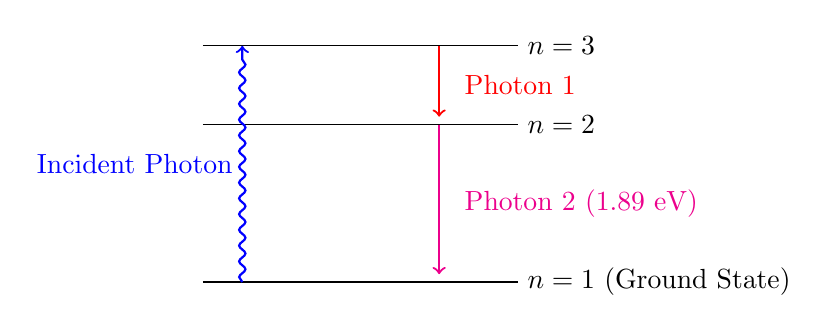
\begin{tikzpicture}
    % Energy levels
    \draw (-2,0) -- (2,0) node[right]{$n=1$ (Ground State)};
    \draw (-2,2) -- (2,2) node[right]{$n=2$};
    \draw (-2,3) -- (2,3) node[right]{$n=3$};
    
    % Excitation
    \draw[->, thick, blue, decorate, decoration={snake,amplitude=0.4mm,segment length=2mm,post length=1mm}] (-1.5,0) -- (-1.5,3);
    \node[left, blue] at (-1.5, 1.5) {Incident Photon};
    
    % De-excitation cascade
    \draw[->, thick, red] (1,3) -- (1,2.1);
    \node[right, red] at (1.2, 2.5) {Photon 1};
    
    \draw[->, thick, magenta] (1,2) -- (1,0.1);
    \node[right, magenta] at (1.2, 1) {Photon 2 (1.89 eV)};
\end{tikzpicture}
\caption{Energy level diagram for the multi-photon emission problem.}
\end{figure}

\textbf{Solution:}
\begin{description}
    \item[(a) Determine Energy Levels:] An energy of 1.89 eV corresponds to the $n=3 \to n=2$ transition in hydrogen. As this was the second photon in the cascade to ground, the path was $n_{excited} \to n=2 \to n=1$. Therefore, the atom was initially excited to the \textbf{n=3 level}.
    \item[(b) Incident Photon Wavelength:] The incident photon caused the $n=1 \to n=3$ excitation.
    $\Delta E_{1 \to 3} = 13.6(1 - 1/9) \approx 12.09$ eV.
    $\lambda = hc/E = 1240 / 12.09 \approx 102.6$ nm.
\end{description}
\textbf{Final Answers:} (a) The atom was excited to the \textbf{n=3} level. (b) The incident photon wavelength was \textbf{102.6 nm}.

\hrulefill
\subsection*{Problem 3: Excitation by Collision and Possible Emissions}
\begin{quote}
A stationary singly ionized helium ion (He$^{+}$) is in a state with orbital angular momentum $L = h/\pi$. It is struck by a proton with 50 eV of kinetic energy. What are the possible wavelengths of light that can be emitted as the ion de-excites?
\end{quote}

\textbf{Solution:}
\begin{enumerate}
    \item \textbf{Initial State:} $L = n(h/2\pi) \implies n=2$.
    \item \textbf{Possible Excitations:} The proton's 50 eV energy is greater than the ionization energy from the n=2 state (13.6 eV), so any higher level is accessible.
    \item \textbf{Possible Emissions:}
    \begin{itemize}
        \item $4 \to 2$: $\Delta E = 10.2$ eV $\implies \lambda \approx \textbf{121.6 nm}$.
        \item $3 \to 2$: $\Delta E \approx 7.56$ eV $\implies \lambda \approx \textbf{164 nm}$.
        \item $2 \to 1$: $\Delta E = 40.8$ eV $\implies \lambda \approx \textbf{30.4 nm}$.
    \end{itemize}
\end{enumerate}
\textbf{Final Answer:} Many wavelengths are possible. Prominent examples include \textbf{121.6 nm}, \textbf{164 nm}, and \textbf{30.4 nm}.

\hrulefill
\subsection*{Problem 4: Head-on Inelastic Collision}
\begin{quote}
A neutron with kinetic energy $K$ collides head-on with a stationary hydrogen atom in its ground state. What is the minimum value of $K$ (in eV) required for the neutron to cause an excitation? [Assume $m_n \approx m_H = m$.]
\end{quote}

\textbf{Solution:}
For minimum initial KE, the collision must be perfectly inelastic (particles stick together).
\begin{enumerate}
    \item \textbf{Momentum Conservation:} $mv_n = (m+m)V \implies V = v_n/2$.
    \item \textbf{Energy Conservation:} $K = \frac{1}{2}(2m)V^2 + \Delta E$.
    \item \textbf{Solve for K:} Substituting $V$ and using $K = \frac{1}{2}mv_n^2$, we get:
    $K = m(v_n/2)^2 + \Delta E = \frac{1}{4}mv_n^2 + \Delta E = \frac{K}{2} + \Delta E \implies K = 2\Delta E$.
    \item \textbf{Calculate Minimum K:} The minimum excitation is $\Delta E_{1 \to 2} = 10.2$ eV.
    $K_{min} = 2 \times 10.2 \text{ eV} = 20.4 \text{ eV}$.
\end{enumerate}
\textbf{Final Answer:} The minimum kinetic energy required is \textbf{20.4 eV}.

\end{document}